\documentclass[APA,LATO1COL]{WileyNJD-v2}
\usepackage{lmodern}
\articletype{Article Type}%

\received{26 April 2016}
\revised{6 June 2016}
\accepted{6 June 2016}

\raggedbottom


\begin{document}


\title{Case-Base Neural Networks: survival analysis with time-varying,
higher-order interactions}

\author[1]{Jesse Islam}

\author[2]{Maxime Turgeon}

\author[3]{Robert Sladek}

\author[4]{Sahir Bhatnagar}



\address[1]{\orgdiv{Department of Quantitative life sciences,} \orgname{McGill University}, \orgaddress{\state{Quebec}, \country{Canada}}}

\address[2]{\orgdiv{Department of Statistics}, \orgname{University of Manitoba}, \orgaddress{\state{Manitoba}, \country{Canada}}}

\address[3]{\orgdiv{Department of Human Genetics}, \orgname{McGill University}, \orgaddress{\state{Quebec}, \country{Canada}}}

\address[4]{\orgdiv{Department of Biostatistics}, \orgname{McGill University}, \orgaddress{\state{Quebec}, \country{Canada}}}

\corres{Jesse Islam's \email{jesse.islam@mail.mcgill.ca}}

\presentaddress{This is sample for present address text this is sample for present address text}

\abstract[Summary]{Neural network-based survival methods can model data-driven
covariate interactions. While these methods have led to better
predictive performance than regression-based approaches, they cannot
model both time-varying interactions and complex baseline hazards. To
address this, we propose Case-Base Neural Networks (CBNN) as a new
approach that combines the case-base sampling framework with flexible
architectures. Our method naturally accounts for censoring and does not
require method specific hyperparameters. Using a novel sampling scheme
and data augmentation, we incorporate time directly into a feed-forward
neural network. CBNN predicts the probability of an event occurring at a
given moment and estimates the hazard function. We compare the
performance of CBNN to survival methods based on regression and neural
networks in a simulation and three real data applications. We report
two time-dependent metrics for each model. In the simulations and real
data applications, CBNN provides a more consistent predictive
performance across time and outperforms the competing neural network
approaches. For a complex simulation, which highlights the ability of
CBNN to model both a complex baseline hazard and time-varying
interactions, CBNN outperforms all competitors. The first two real data
application shows CBNN outperforming all neural network competitors,
while a second real data application shows competitive performance.
We highlight the benefit of combining case-base sampling with deep
learning to provide a simple and flexible modeling framework for
data-driven, time-varying interaction modeling of
survival outcomes. An R package is available at
\url{https://github.com/Jesse-Islam/cbnn}.}

\keywords{survival analysis, machine learning, case-base, neural
network}



\maketitle




\hypertarget{introduction}{%
\section{Introduction}\label{introduction}}

Smooth-in-time accelerated failure time (AFT) models can estimate
absolute risks by modeling the hazard directly through a user-specified
baseline hazard distribution \citep{kleinbaum2012survival}. Cox
proportional hazards models are used more often than AFT models, causing
analyses to be based on hazard ratios and relative risks rather than on
survival curves and absolute risks \citep{hanley2009}. The
identification of an appropriate distribution for the baseline hazard in
an AFT model may be difficult for common diseases that have many
interacting risk factors, or a Cox model where the disease pathogenesis
may change with age, making it difficult to maintain the proportional
hazards assumption. For example, previous studies of breast cancer
incidence have discovered time-varying interactions with covariates of
interest, such as tumor size \citep{coradini2000time}. One approach to
provide flexibility in the baseline hazard involves using the basis of
splines on time in our model \citep{royston2002flexible}. However,
regression-based models are limited in that they require prior knowledge
about potential time-varying interactions and their quantitative
effects.

Neural networks provide a data-driven approach to approximating
interaction terms. For example, DeepSurv is a neural network-based
proportional hazards model that implements the Cox partial
log-likelihood as a custom loss function \citep{katzman2018DeepSurv},
resulting in a stepwise absolute risk curve that cannot accommodate
time-varying interactions. Compared to Cox regression, DeepSurv shows
better performance on a real dataset \citep{katzman2018DeepSurv}. To handle
non-proportional hazards, a modification to the loss function was
proposed \citep{faraggi1995neural}. 

As an alternative method that assumes a baseline hazard distribution,
DeepHit specifies each survival time of interest in the model and
directly estimates survival curves, rather than deriving a hazard
function . It assumes an inverse Gaussian
distribution as the baseline hazard and it outperformed DeepSurv \citep{lee2018DeepHit}.

Providing further flexibility, Deep Survival Machines (DSM) is a
parametric survival model using neural networks with a mixture of
distributions as the baseline hazard \citep{dsmPaper}. DSM outperformed DeepSurv and DeepHit
\citep{dsmPaper}. However, like DeepHit and DeepSurv, DSM cannot model
time-varying interactions.

We note that these alternative neural network approaches all require
custom loss functions \citep{katzman2018DeepSurv} \citep{lee2018DeepHit}
\citep{dsmPaper}. DeepHit introduces a hyperparameter weighing its two
loss functions (negative log-likelihood and ranking losses) while DSM
requires a two-phase learning process and user implementations for
distributions beyond Log-Normal or Weibull \citep{lee2018DeepHit}
\citep{dsmPaper}. Regression-based approaches require prior
specification of all interaction terms, which makes it challenging to
model covariate effects that change over time. The current neural
network models provide flexibility at the cost of opacity, while
regression models provide clarity at the cost of flexibility.

In this article, we propose Case-Base Neural Networks (CBNN) as a method
that models time-varying interactions and a flexible baseline hazard
using commonly available neural network components. Our approach to
modeling the full hazard uses case-base sampling \citep{hanley2009}.
This sampling technique allows probabilistic models to predict survival
outcomes. As part of the case-base framework, we use transformations of
time as a feature (covariate) to specify different baseline hazards. For
example, by including splines of time as covariates, we can approximate
the Royston-Parmar flexible baseline hazard model
\citep{royston2002flexible}, however, this still requires explicit use
of time-varying interactions. CBNN can model both without extra tuning
parameters.

In Section \ref{methods}, we describe how case-base sampling and neural
networks are combined both conceptually and algebraically, along with
our hyperparameter choices and software implementation. Section
\ref{sims}, describes our metrics and compares the performance of CBNN,
DeepSurv, DeepHit, DSM, Cox regression and case-base using logistic
regression (CBLR) on simulated data. Section \ref{casestudies} describes
the real-data analysis, while Section \ref{discussion} explores the
implications of our results and contextualizes them within neural
network survival analysis in a single event setting.



%%%%%%%%%%%%%%%%%%%%%%%%%%%%%%%%%%%%%%%%%%%%%%
%%%%%%%%%%%%%%%%%%%%%%%%%%%%%%%%%%%%%%%%%%%%%%
%%%%%%%%section2
%%%%%%%%%%%%%%%%%%%%%%%%%%%%%%%%%%%%%%%%%%%%%%
%%%%%%%%%%%%%%%%%%%%%%%%%%%%%%%%%%%%%%%%%%%%%%

\hypertarget{methods}{%
\section{Case-base neural network methodology, metrics and
software}\label{methods}}

In this section, we define case-base sampling, which converts the total
survival time into discrete person-specific moments (person-moments).
Then, we detail how neural networks can be used within this framework,
explicitly incorporating time as a feature while adjusting for the
sampling bias. Finally, we report on the software versions used. An R
package is available for use at
\url{https://github.com/Jesse-Islam/cbnn}. The entire code base to
reproduce the figures and empirical results in this paper is available
at \url{https://github.com/Jesse-Islam/cbnnManuscript}.

\hypertarget{case-base-sampling}{%
\subsection{Case-base sampling}\label{case-base-sampling}}

Case-base sampling is an alternative framework for survival analysis
\citep{hanley2009}. In case-base sampling, we sample from the continuous
survival time of each person in our dataset to create a \emph{base
series} of \emph{person-moments}. This \emph{base series} complements
the \emph{case series}, which contains all person-moments at which the
event of interest occurs.

For each person-moment sampled, let \(X_i\) be the corresponding
covariate profile \(\left(x_{i1},x_{i2},...,x_{ip} \right)\), \(T_i\) be
the time of the person-moment and \(Y_i\) be the indicator variable for
whether the event of interest occurred at time \(T_i\). We estimate the
hazard function \(h(t \mid X_i)\) using the sampled person-moments.
Recall that \(h(t \mid X_i)\) is the instantaneous potential of
experiencing the event at time \(t\) for a given set of covariates
\(X_i\), assuming \(T_i \geq t\).

Now, let \(b\) be the (user-defined) size of the \emph{base series} and
let \(B\) be the sum of all follow-up times for the individuals in the
study. If we sample the \emph{base series} uniformly across the study
base, then the hazard function of the sampling process is equal to
\(b/B\). Therefore, we have the following equality
\footnote{We are abusing notation here, conflating hazards with probabilities. For a rigorous treatment, see Saarela \& Hanley (2015) section 3 \cite{saarela2015} .}:
\begin{align}\label{eqn:main}
\frac{P\left(Y_i=1 \mid X_i, T_i\right)}{P\left(Y_i = 0 \mid X_i, T_i\right)} = \frac{h\left(T_i \mid X_i\right)}{b/B}.
\end{align} The odds of a person-moment being a part of the \emph{case
series} is the ratio of the hazard \(h(T_i \mid X_i)\) and the uniform
rate \(b/B\). Using \eqref{eqn:main}, we can see how the log-hazard
function can be estimated from the log-odds arising from case-base
sampling: \begin{align}\label{eqn:offset}
\log \left( h\left(t \mid X_i\right)\right) = \log \left(\frac{P\left(Y_i = 1 \mid X_i, t\right)}{P\left(Y_i = 0 \mid X_i, t\right)}\right) + \log\left(\frac{b}{B}\right).
\end{align}

To estimate the correct hazard function, we adjusting for the bias
introduced when sampling a fraction of the study base \(B\) by adding
the offset term \(\log\left(\frac{b}{B} \right)\) as in
\eqref{eqn:offset}. Next, we propose using neural networks to model the
odds.

\hypertarget{neural-networks-to-model-the-hazard-function}{%
\subsection{Neural networks to model the hazard
function}\label{neural-networks-to-model-the-hazard-function}}

After case-base sampling, we pass all features, including time, into any
user-defined feed-forward component, to which an offset term is added,
then passed through a sigmoid activation function (Figure
\ref{fig:NNarch}). We use the sigmoid function as its inverse is the
odds, which we can use to calculate the hazard. The general form for the
neural network using CBNN is:

\begin{align}\label{eqn:nnProb}
P\left(Y=1|X,T\right)&=\mathrm{sigmoid}\left(f_{\theta}(X, T) + \log\left(\frac{B}{b}\right) \right),
\end{align}

where \(T\) is a random variable representing the event time, \(X\) is
the random variable for a covariate profile, \(f_{\theta}(X, T)\)
represents any feed-forward neural network architecture,
\(\log\left(\frac{B}{b}\right)\) is bias term set by case-base sampling,
\(\theta\) is the set of parameters learned by the neural network and
\(\mathrm{sigmoid}(x)=\frac{1}{1+e^{-x}}\). By approximating a
higher-order polynomial of time using a neural network, the baseline
hazard specification is now data-driven, where user-defined
hyperparameters such as regularization, number of layers and nodes
control the flexibility of the hazard function. We provide a detailed
description of the choices we made in the next sub-section.

\begin{figure}

{\centering 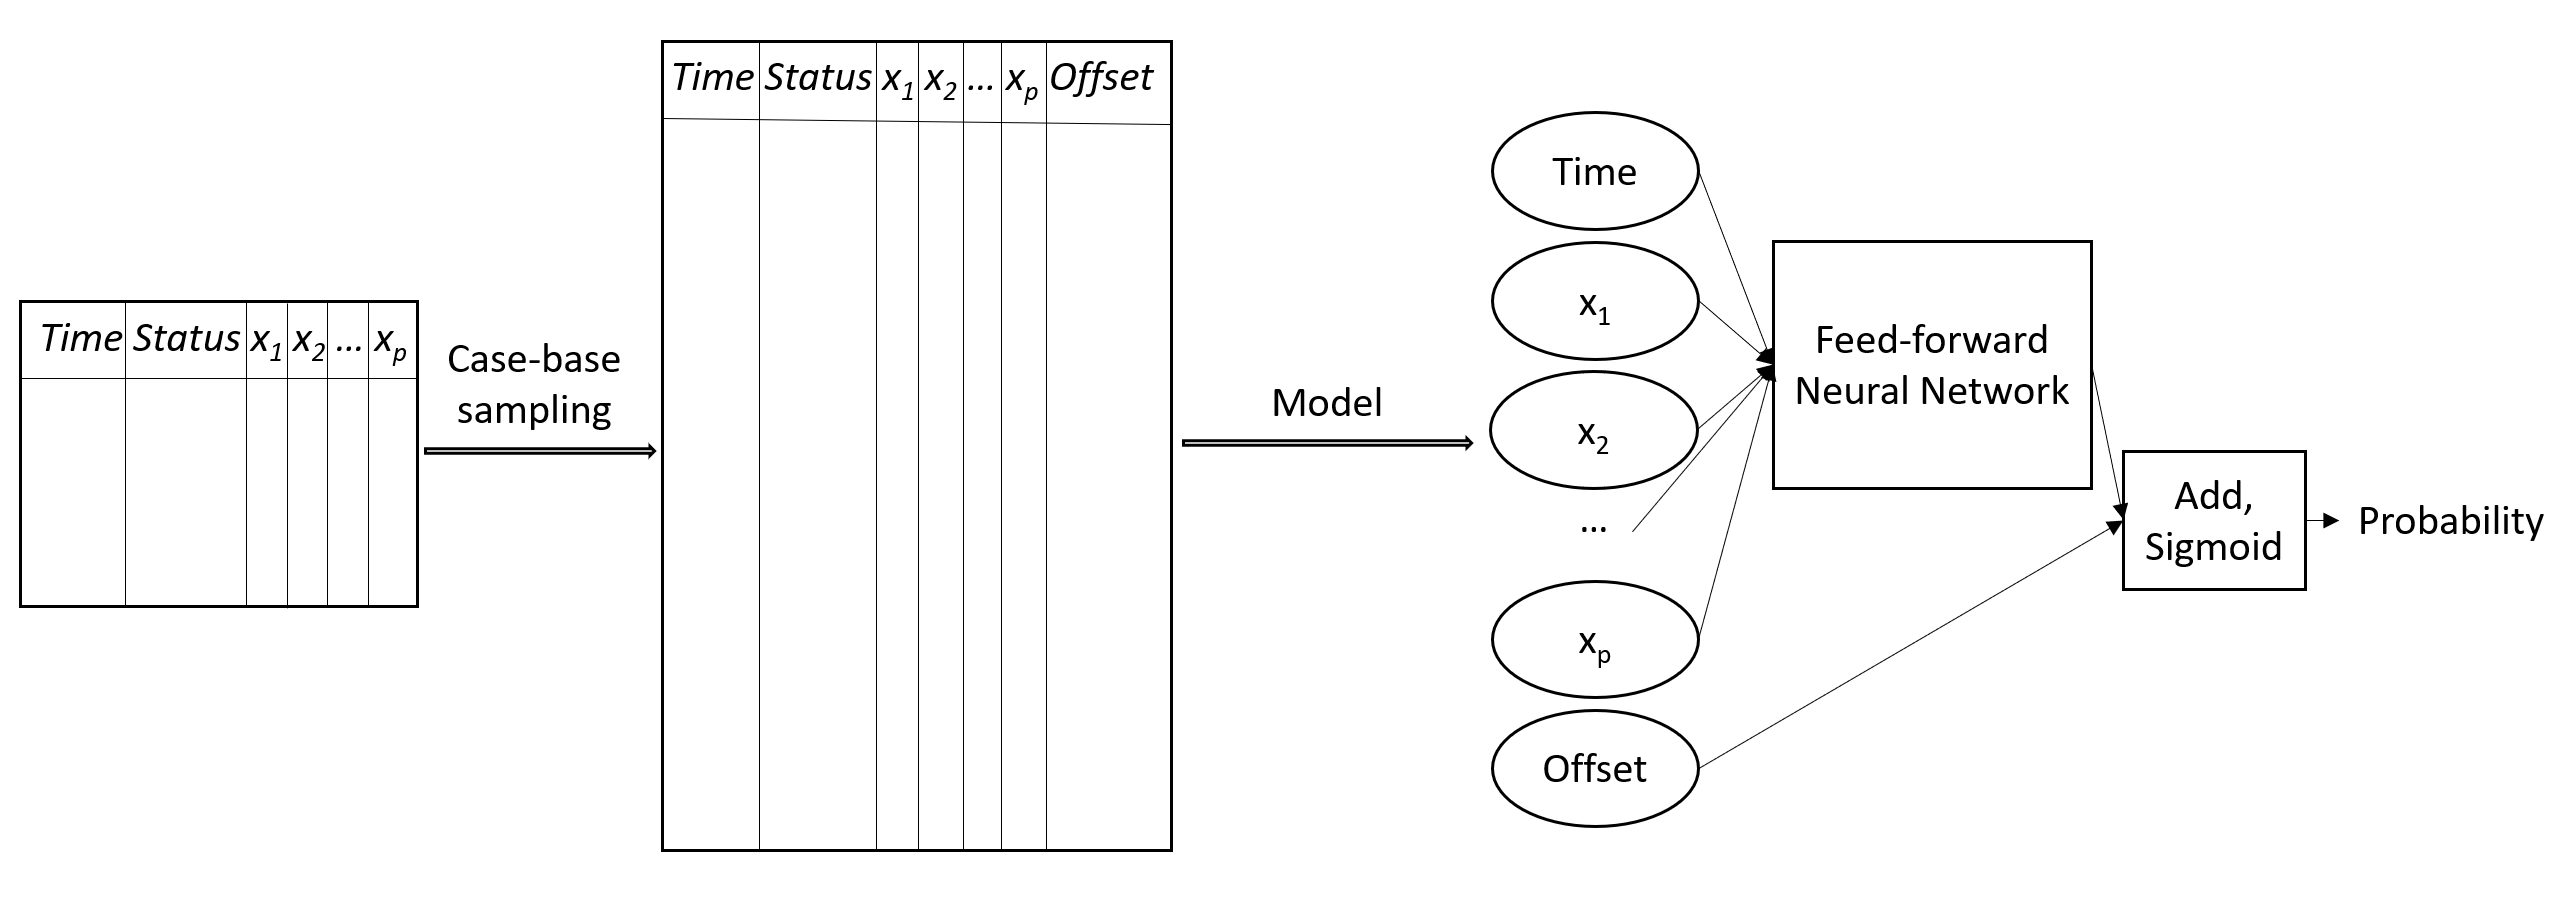
\includegraphics[width=1\linewidth]{../../../figures/nnarch2}}

\caption{Steps involved in CBNN from case-base sampling to the model framework we use for training. The first step is case-base sampling, completed before training begins. Next, we pass this sampled data through a feed-forward neural network. We add the offset and pass that through a sigmoid activation function, whose output is a probability. Once the neural network model completes its training, we can convert the probability output to a hazard, using it for our survival outcomes of interest.}\label{fig:NNarch}
\end{figure}

The following derivation shows how our probability estimate is converted
to odds: \begin{align*}
 \log\left( h(t \mid X) \right) &= \log\left(\frac{\mathrm{sigmoid}\left(f_{\theta}(X, T) + \log\left(\frac{B}{b}\right)\right)}{1-\mathrm{sigmoid}\left(f_{\theta}(X, T) + \log\left(\frac{B}{b}\right)\right)}\right) + \log\left(\frac{b}{B}\right) \\
 &= \log\left( \frac{\frac{\exp\left(f_{\theta}(X, T) + \log\left(\frac{B}{b}\right)\right)}{\exp\left(f_{\theta}(X, T) + \log\left(\frac{B}{b}\right)\right)+1}}{1-\frac{\exp\left(f_{\theta}(X, T) + \log\left(\frac{B}{b}\right)\right)}{\exp\left(f_{\theta}(X, T) + \log\left(\frac{B}{b}\right)\right)+1}}\right) + \log\left(\frac{b}{B}\right) \\
 &= \log\left(\exp\left( f_{\theta}(X, T) + \log\left(\frac{B}{b}\right) \right) \right) + \log\left(\frac{b}{B}\right) \\
 &= f_{\theta}(X, T) + \log\left(\frac{B}{b}\right) + \log\left(\frac{b}{B}\right) \\
&= f_{\theta}(X, T). 
\end{align*}

We use binary cross-entropy as our loss function \citep{gulli2017}:
\begin{align*}
L(\theta)=-\frac{1}{N} \sum^{N}_{i=1} y_{i} \cdot \log(\hat{f}_{\theta}(x_{i}, t_{i}) ) + (1-y_{i} )\cdot \log(1-\hat{f}_{\theta}(x_{i}, t_{i}) ),
\end{align*} where \(\hat{f}_{\theta}(x_{i}, t_{i})\) is our estimate
for a given covariate profile and time, \(y_{i}\) is our target value
specifying whether an event occurred and \(N\) represents the number of
individuals in our training set.

Backpropagation with an appropriate minimization algorithm (e.g.~Adam,
RMSPropagation, stochastic gradient descent) is used to optimize the
parameters in the model \citep{gulli2017}. For our analysis, we use Adam
as implemented in Keras \citep{gulli2017}. Note that the size of the
\emph{case series} is fixed as the number of events, but we can make the
\emph{base series} as large as we want. A ratio of 100:1 \emph{base
series} to \emph{case series} is sufficient \citep{hanley2009}. We pass
our feed-forward neural network through a sigmoid activation function
(Figure \ref{fig:NNarch}). Finally, we can convert this model output to
a hazard. When using our model for predictions, we manually set the
offset term to 0 in the new data, as we account for the bias during the
fitting process.

Since we are directly modeling the hazard, we can readily estimate the
risk function (\(F\)) at time \(t\) for a covariate profile \(X\),
viz.\begin{align}\label{eqn:ci2}
F\left(t\mid X\right)& = 1 - \exp\left(-\int_{0}^{t}h(u|X) \,\textrm du\right).
\end{align} We use a finite Riemann sum \citep{hughes2020calculus} to
approximate the integral in \eqref{eqn:ci2}.

\hypertarget{hyperparameter-selection}{%
\subsection{Hyperparameter selection}\label{hyperparameter-selection}}

Neural networks are flexible when defining the architecture and
optimization parameters. These hyperparameter choices can affect the
estimated parameters and are not necessarily the same for each model.
First we fix a test set with 15\% of the data, then we use three-fold cross-validation on the remaining 
data (85\%:15\% training:validation) for a range of hyperparameters (TABLE REF). We track integrated brier 
score on the validation set for each hyperparameter combination, choosing 
the combination with the lowest score for each method. The chosen 
hyperparameters are in (TABLE REF).

\hypertarget{software-implementation}{%
\subsection{Software implementation}\label{software-implementation}}

R \citep{Rsoft} and python \citep{py} are used to evaluate methods from
both languages. We fit the Cox model using the \textbf{survival} package
\citep{survpkg}, the CBLR model using the \textbf{casebase} package
\citep{cbpkg}, the DeepSurv model using the \textbf{survivalmodels}
package \citep{survmods}, the DeepHit model using \textbf{pycox}
\citep{lee2018DeepHit} and the DSM model using
\textbf{DeepSurvivalMachines} \citep{dsmPaper}. We made the components
of CBNN using the \textbf{casebase} package for the sampling step and
the \textbf{keras} \citep{keras} package for our neural network
architecture. The \textbf{simsurv} package \citep{simsurv} is used for
our simulation studies, while \textbf{flexsurv} \citep{flexsurv} is used
to fit a flexible baseline hazard using splines for our complex
simulation. We use the implementation of \(C_{IPCW}\) from the python
package \textbf{sksurv} \citep{sksurv}. The \textbf{riskRegression}
package \citep{riskRegression} is used to get the Index of Prediction
Accuracy (IPA metric). Both metrics are described in detail in the
following section. We modify the \textbf{riskRegression} package to be
used with any user supplied risk function \(F\). To ensure that both R
and Python-based models are running in unison on the same data through
our simulations and bootstrap, we use the \textbf{reticulate} package
\citep{reticulate}.



%%%%%%%%%%%%%%%%%%%%%%%%%%%%%%%%%%%%%%%%%%%%%%
%%%%%%%%%%%%%%%%%%%%%%%%%%%%%%%%%%%%%%%%%%%%%%
%%%%%%%%section3
%%%%%%%%%%%%%%%%%%%%%%%%%%%%%%%%%%%%%%%%%%%%%%
%%%%%%%%%%%%%%%%%%%%%%%%%%%%%%%%%%%%%%%%%%%%%%




\hypertarget{performance-metrics}{%
\section{Performance metrics}\label{performance-metrics}}

To choose our method-specific hyperparameters, we use the Integrated 
Brier Score (IBS) \citep{graf1999}. We use two metrics to assess the 
performance of the different methods of interest on testing data: 1) (IPA) 
\citep{kattan2018index} and 2) inverse probability
censoring weights-adjusted concordance index (\(C_{IPCW}\))
\citep{uno2011}, which we define below. IBS provides a summarized assessment
of performance for each model. (\(C_{IPCW}\)) provides information
about performance up to the survival time of interest. while IPA provide transparency
as to when in follow-up time each model may
perform better than the others.


\hypertarget{index-of-prediction-accuracy-ipa}{%
\subsubsection{Index of prediction accuracy (IPA)}\label{index-of-prediction-accuracy-ipa}}

The IPA is a function of the Brier score (\(BS(t)\)) \citep{graf1999},
which is defined as \begin{align}
BS(t)=\frac{1}{N}\sum^{N}_{i=1}\left(\frac{\left(1 - \widehat{F}(t \mid X_{i})\right)^{2}\cdot I(T_{i}\leq t,\delta_{i}=1)}{\widehat{G}(T_{i})} + \frac{\widehat{F}(t\mid X_{i})^{2}\cdot I(T_{i}>t)}{\widehat{G}(t)}\right),
\end{align} where \(\delta_{i}=1\) shows individuals who have
experienced the event, \(N\) represents the number of samples in our
dataset over which we calculate \(BS(t)\), \(\widehat{G}(t)=P[c>t]\) is
a non-parametric estimate of the censoring distribution, \(c\) is
censoring time and \(T_{i}\) is an individual's survival or censoring
time. The Brier score provides a score that accounts for the information
loss because of censoring. There are three categories of individuals
that may appear within the dataset once we fix our \(t\) of interest.
Individuals who experienced the event before \(t\) are present in the
first term of the equation. The second term of the equation includes
individuals who experience the event or are censored after \(t\). Those
censored before \(t\) are the third category of people. The inverse
probability censoring weights (IPCW) adjustment (\(G(\cdot)\)) is to
account for these category three individuals whose information is
missing. The IPA score as a function of time is given by \begin{align}
\textrm{IPA}(t) &= 1-\frac{BS_{model}(t)}{BS_{null}(t)}, \nonumber
\end{align} where \(BS_{model}(t)\) represents the Brier score over time
\(t\) for the model of interest and \(BS_{null}(t)\) represents the
Brier score if we use an unadjusted Kaplan-Meier (KM) curve as the
prediction for all observations \citep{kattan2018index}. Note that IPA
has an upper bound of one, where positive values show an increase in
performance over the null model and negative values show that the null
model performs better. These scores show how performance changes over
follow-up time.

A potential artifact of IPA is that the score is unstable at earlier and
later survival times. This is because of a near equivalent Brier score
among each model and the null model. At small values, a difference of
\(0.1\) creates a more significant fold change than at larger values. As
the Brier score is potentially small at the start and at the end of
their respective curves, The IPA score may be unstable at the same
locations.

\hypertarget{integrated-brier-score-ibs}{%
\subsubsection{Integrated Brier Score (IBS)}\label{integrated-brier-score-ibs}}

The IBS is a function of the Brier score (\(BS(t)\)) \citep{graf1999}. as well,
which is defined as \begin{align}
IBS=\int_{t}^{t_{max}}BS(t)dw(t)
\end{align} where $w(t)=\frac{t}{t_{max}}$. As this is a score for a range of follow-up-time,
it is a useful metric to track during cross-validation. The performance at a specific time
is hidden, and is why we opt for the IPA in assessing the final models on a test set.

\hypertarget{inverse-probability-censoring-weights-adjusted-concordance-index}{%
\subsubsection{Inverse probability censoring weights-adjusted
concordance
index}\label{inverse-probability-censoring-weights-adjusted-concordance-index}}

The \(C_{IPCW}\) is a non-proper, rank-based metric that does not depend
on the censoring times in the test data \citep{uno2011}. The
\(C_{IPCW}\) is given by

\begin{align} \label{eq:cidx}
C_{IPCW}(t) &= \frac{\sum^{N}_{i=1}\sum^{N}_{j=1}\delta_{i}\left\{\widehat{G}(T_{i})\right\}^{-2} I(T_{i}<T_{j},T_{i}<t) I\left(\widehat{F}(t|X_{i})>\widehat{F}(t|X_{j})\right)}{\sum^{N}_{i=1}\sum^{N}_{j=1}\delta_{i}\left\{\widehat{G}(T_{i})\right\}^{-2} I(T_{i}<T_{j},T_{i}<t)}.
\end{align} where the follow-up period of interest is (0,\(t\)),
\(I(\cdot)\) is an indicator function, \(\widehat{F}(X_{i},t)\) is the
risk function estimated for everyone in the study at time \(t\) and
\(C_{IPCW}\) can compare the performance of different models, where a
higher score is better. Note that the \(C_{IPCW}\) may produce
misleading performance, as it ranks based on survival times, not event
status \citep{cindexfails2019}. This metric is considered an unbiased
population concordance measure because of the IPCW adjustment
\citep{uno2011}.

\begin{figure}

{\centering 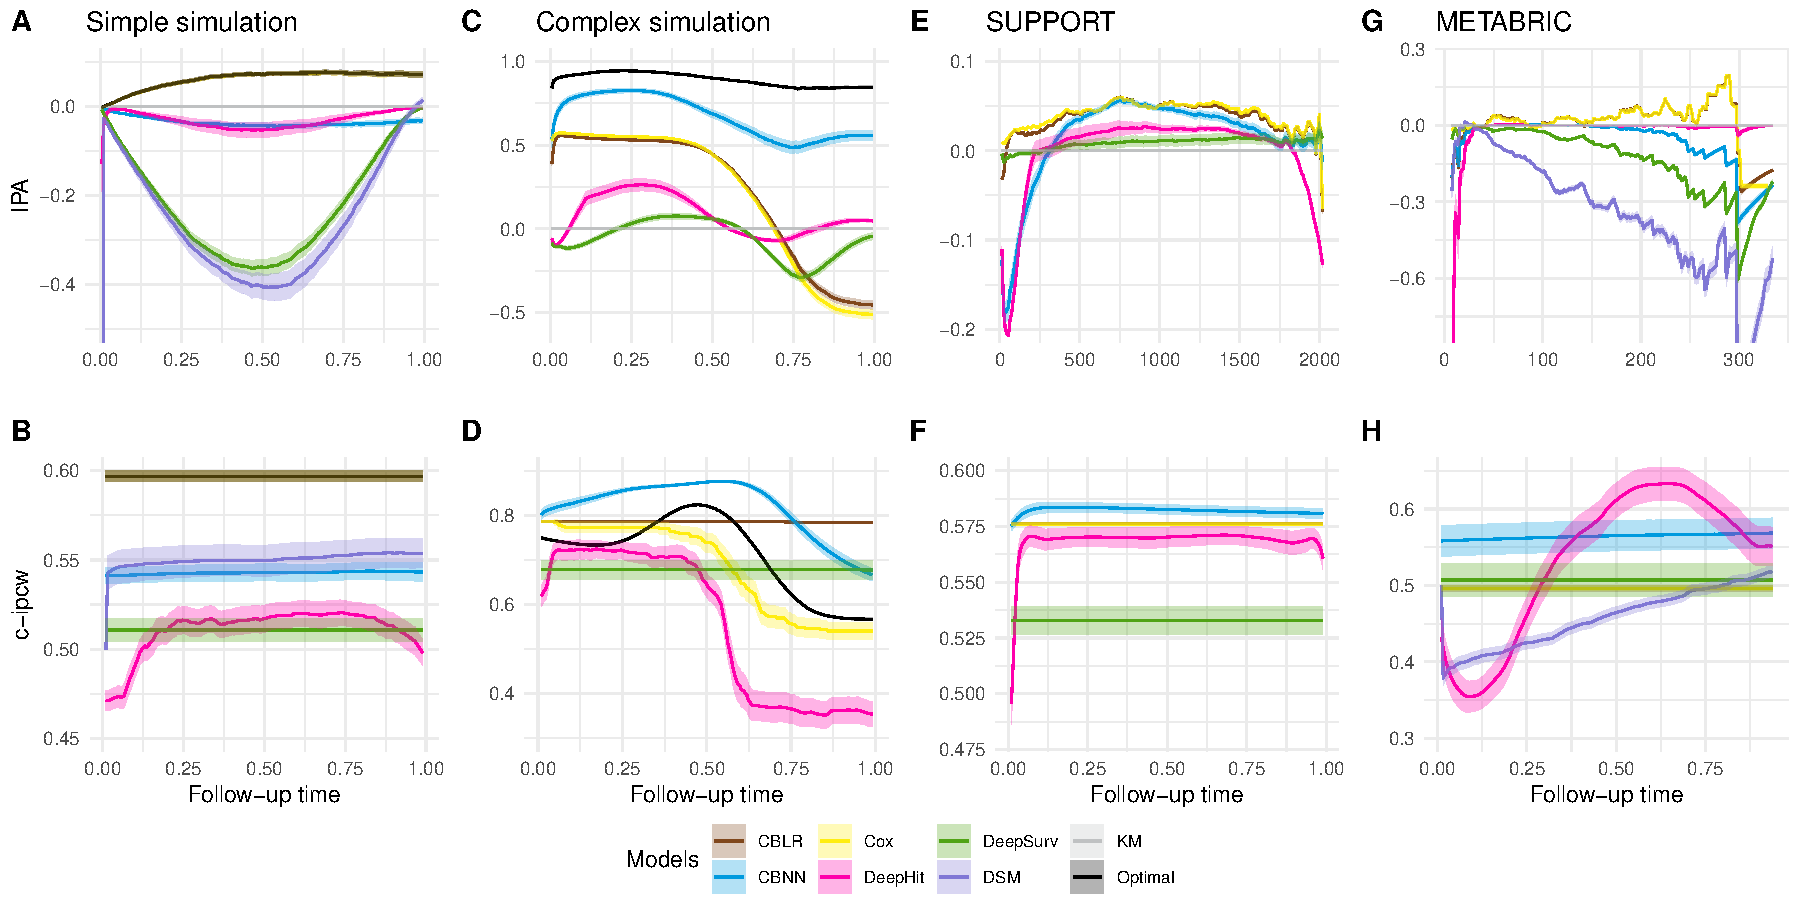
\includegraphics[width=1\linewidth]{../../../analyses/figures/megaPlot} 

}

\caption{Summarizes the simple simulation (A, B), complex simulation (C, D), SUPPORT case study (E, F) and METABRIC case study (G, H) results. The first row shows the IPA score for each model in each study over follow-up time. Negative values mean our model performs worse than the null model and positive values mean the model performs better. The second row demonstrates the $C_{IPCW}$ score for each model in each study over follow-up time. A score of 1 is the maximum performance for either metric. Each model-specific metric in each study shows a 95-percent confidence interval over 100 iterations. The models of interest are case-base with logistic regression (CBLR), Case-Base Neural Networks (CBNN), Cox, DeepHit, DeepSurv, Deep Survival Machines (DSM), Optimal (a CBLR model with the exact interaction terms and baseline hazard specified) and Kaplan-Meier (to serve as a baseline, predicting the average for all individuals).}\label{fig:megaPlot}
\end{figure}

\hypertarget{sims}{%
\section{Simulation study}\label{sims}}

In this section, we simulate data to evaluate the performance of
CBNN and compare our approach with existing regression-based (Cox, CBLR)
and neural network-based (DeepHit, DeepSurv) methods. We specify a
linear combination of each covariate as the linear predictor in
regression-based approaches (Cox, CBLR), which contrasts with neural
network approaches that allow for non-linear interactions. We simulate
data under a complex baseline hazard with
time-varying interactions, each with 10\% random censoring. For both
settings, we simulate three covariates:

\[
z_{1} \sim \textrm{Bernoulli}(0.5) \qquad \qquad %technically a control and treatement group
z_{2} \sim \begin{cases}
 N(0,0.5) & \textrm{if } z_{1}=0\\ 
 N(1,0.5) & \textrm{if } z_{1}=1
\end{cases} \qquad \qquad
z_{3} \sim N(1,0.5)
\]
Besides the methods mentioned above, we include the Optimal model in our
comparisons using CBLR. That is, we include the exact functional form of
the covariates in a CBLR model (referred to as Optimal for simplicity).
We calculate \(t\)-based 95\% confidence intervals using 100
replications of the simulated data. For all analyses, 15\% of the data is 
kept for testing, while 15\% of the remaining data is kept for validation. 
The remaining data is kept for training. We predict risk functions \(F\) using
\eqref{eqn:ci2} for individuals in the test set, which are used to
calculate our \(C_{IPCW}\) and IPA scores. We conduct 100 bootstrap
re-samples on the training data to obtain confidence intervals.

\hypertarget{complex-simulation-flexible-baseline-hazard-time-varying-interactions}{%
\subsection{Complex simulation: flexible baseline hazard, time-varying
interactions}\label{complex-simulation-flexible-baseline-hazard-time-varying-interactions}}

This simulation demonstrates performance with the presence of a complex
baseline hazard and a time-varying interaction. Inspired by a cancer treatment 
that initially reduces risk of death, but slowly returns as time progresses. 
Originally used to show the spline-based hazard model proposed by Royston and Parmar
\citep{royston2002flexible}, the breast cancer dataset provides a
complex hazard from which we simulate, available in the
\textbf{flexsurv} R package \citep{flexsurv}. To increase the complexity
of our data-generating mechanism for this simulation, we design the
model as follows: \begin{align}
\log h(t \mid X_i) =\sum_{i=1}^{5} (\gamma_{i} \cdot \psi_{i}) + \beta_{{1}} (z_{1}) + \beta_{{2}} (z_{2})+ \beta_{{3}} (z_{3})+ \tau_{1} ( z_{1} \cdot t)+ \tau_{2} (z_{2} \cdot z_{3}), \nonumber
\end{align}


\begin{table}
\caption{Four tables representing performance at certain follow-up times for the simple simulation, complex simulation, SUPPORT and METABRIC. Each table shows performance for each method in each study at $25\%$, $50\%$. $75\%$ and $100\%$ of follow-up time. The bold elements show the best model for each study, at each follow-up time of interest. These tables are included to provide exact measures at certain intervals. The models of interest are: Cox, case-base with logistic regression (CBLR), DeepSurv, DeepHit, Case-Base Neural Network (CBNN) and Optimal}
\label{tab:megaTable}

\begin{center}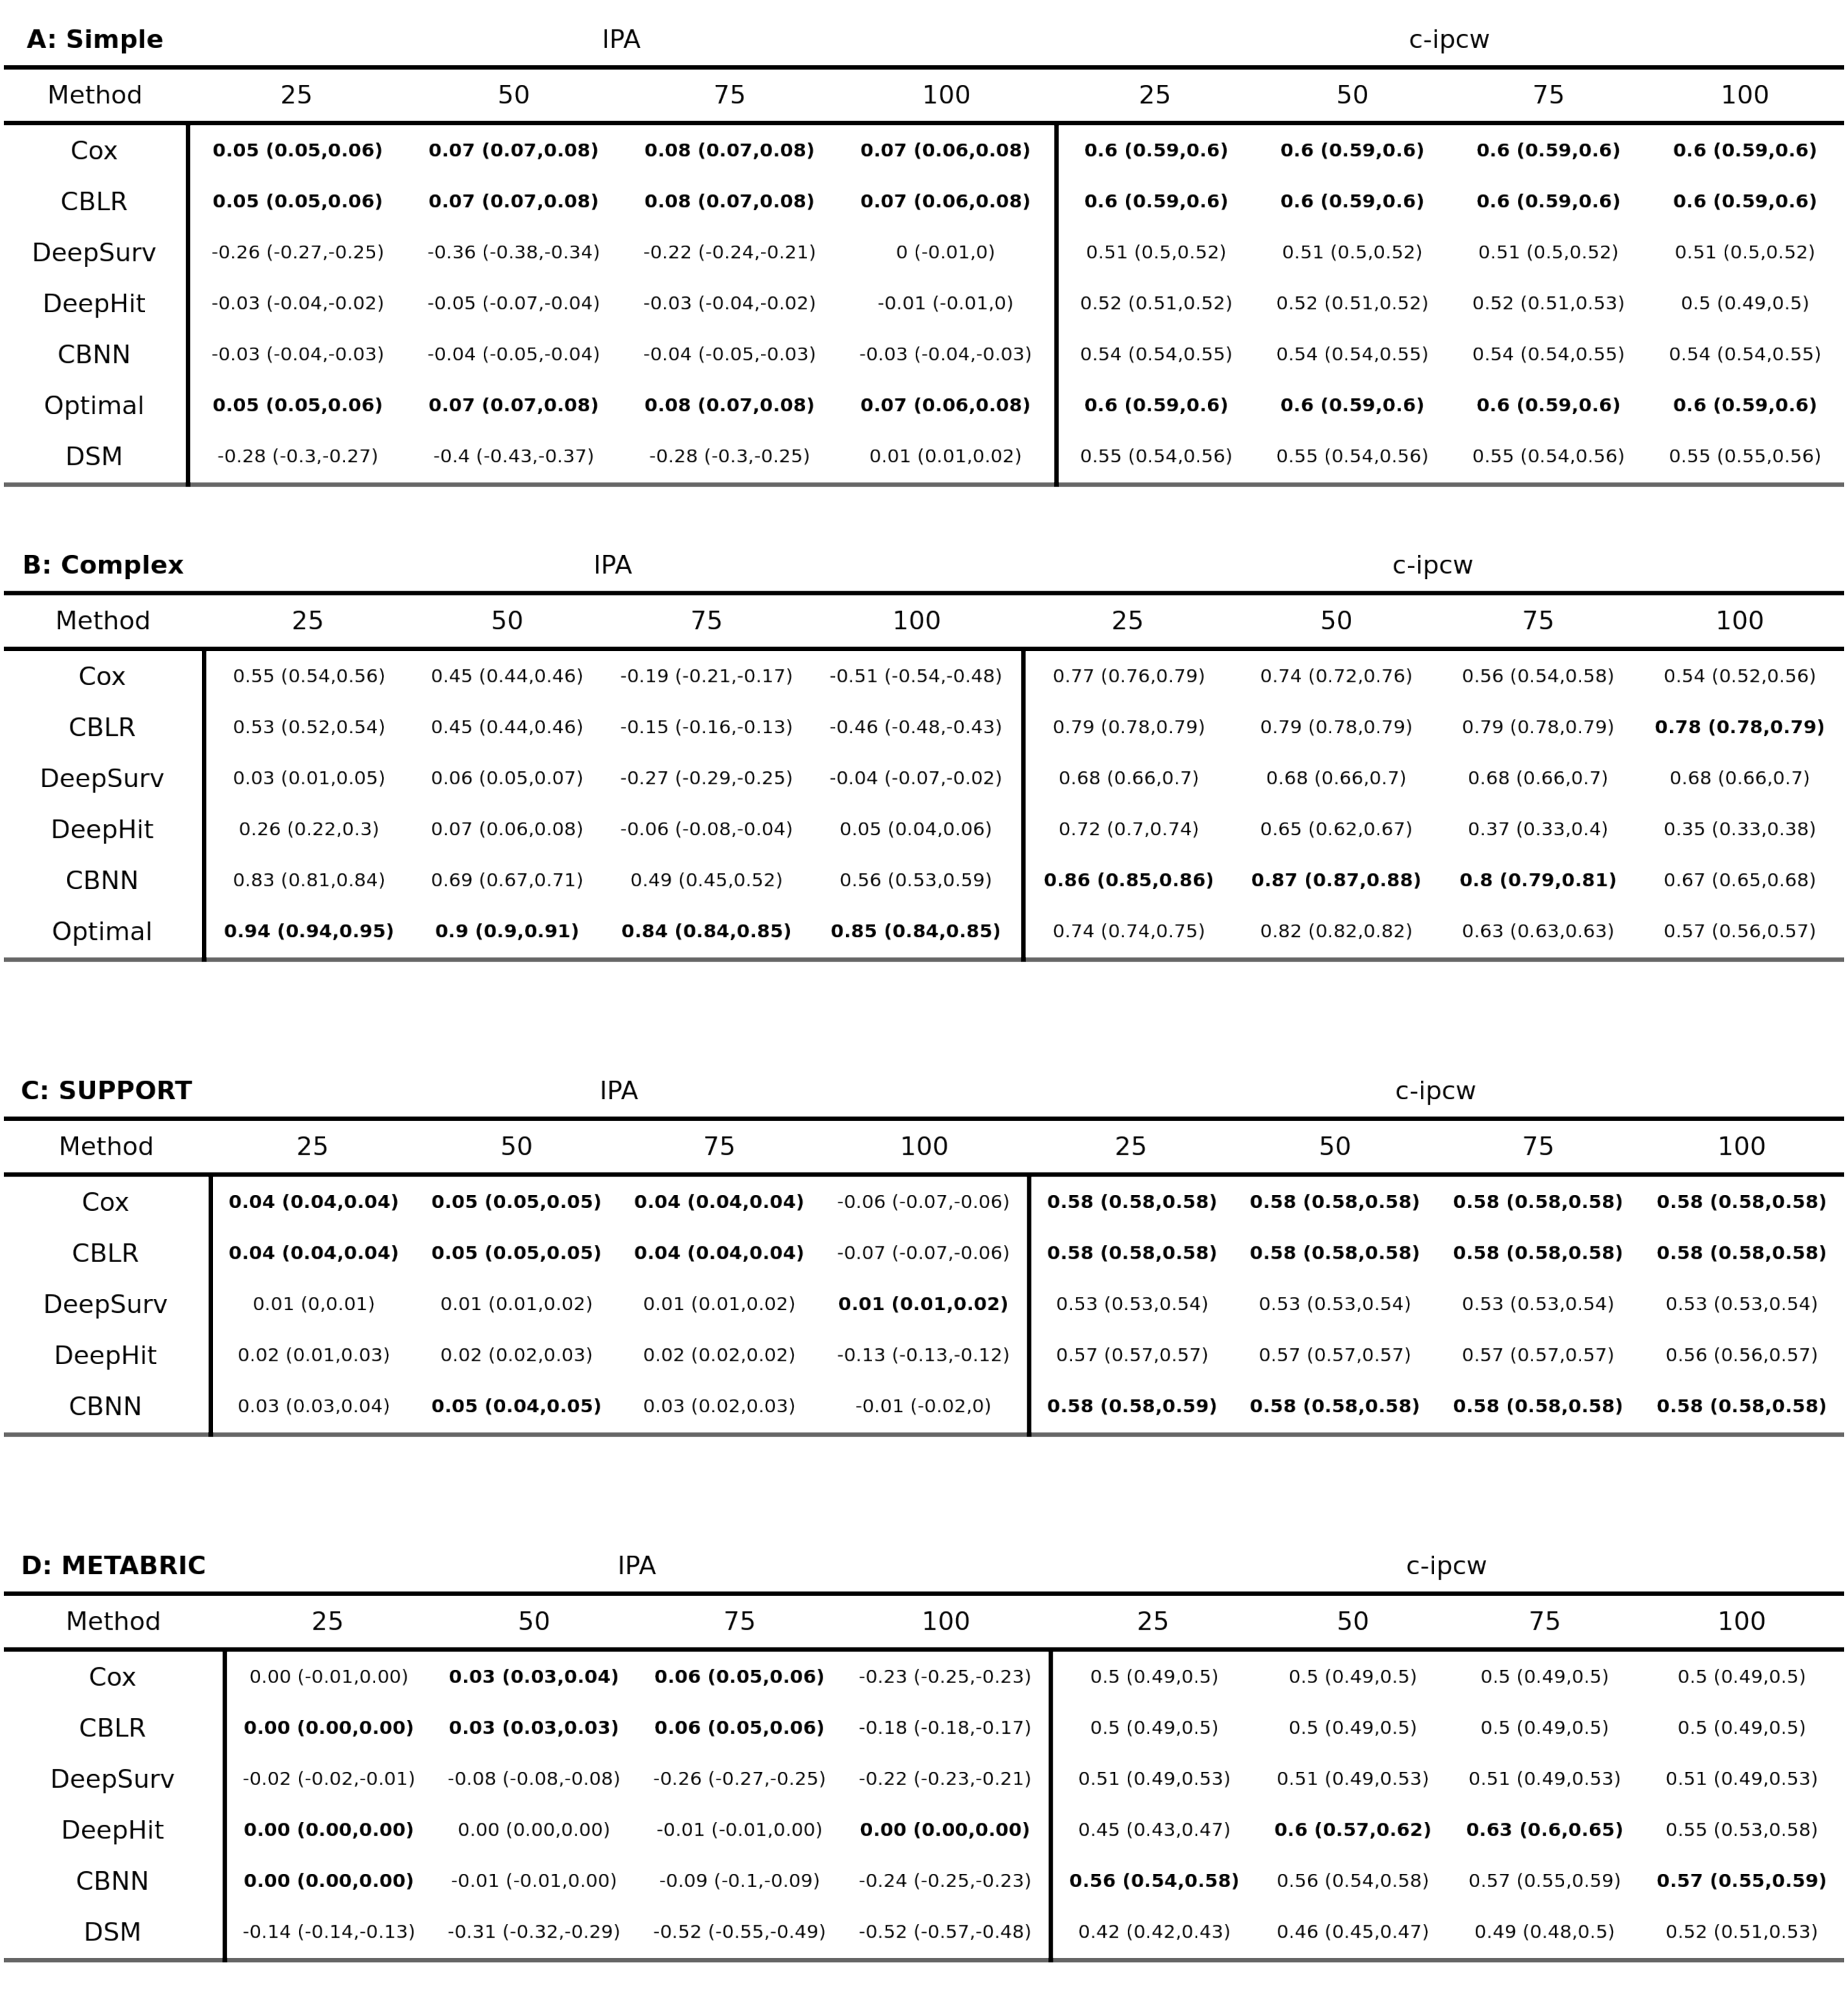
\includegraphics[width=1\linewidth]{../../../analyses/figures/megaTable} \end{center}

\end{table}


where
\(\gamma_{1}=3.9, \gamma_{2}=3, \gamma_{3}=-0.43, \gamma_{4}=1.33,\gamma_{5}=-0.86, \beta_{{1}}=-5, \beta_{{2}}=-1, \beta_{{3}}=1, \tau_{1}=0.001, \tau_{2}=-1\)
and \(\psi\) are basis splines. The \(gamma\) coefficients are obtained
from an intercept-only cubic splines model with three knots using the
\emph{flexsurvspline} function from the \textbf{flexsurv} package
\citep{flexsurv}. Note that we fix these values for the analysis. The
\(\beta\) coefficients represent direct effects, \(\tau_{2}\) and
\({\tau_3}\) represent interactions and \(\tau_{1}\) is a time-varying
interaction.

We use a population time plot to visualize incidence density across $z1$ (FIGURE REF).
z1 acts to mimic a treatment and control group. The control group $(z1=0)$ is not impacted
by the time-varying interaction. The treatment group $(z1=1)$ initially acts to protect the group,
while the risk slowly builds with time at the rate of the interaction term $(\tau_{1})$. This creates
a separation between the median time of death between these two groups due to the time-varying
interaction. We expect all competing models (aside from the Optimal model and CBNN) to drop in
performance for the second half of follow-up time.

\hypertarget{performance-comparison-in-complex-simulation}{%
\subsubsection{Performance comparison in complex
simulation}\label{performance-comparison-in-complex-simulation}}


Figure \ref{fig:megaPlot} A, E and Table \ref{tab:megaTable} A
demonstrates the performance over time on a test set. While examining the IPA score, the optimal
regression model and CBNN perform near identically, leading in performance followed by 
DeepHit, the linear regression models and DeepSurv. We expected the Optimal model to perform best in both
metrics. However, this was not the case for \(C_{IPCW}\) and may be due
to an artifact of concordance-based metrics, where a misspecified model
may perform better than a correctly specified one
\citep{cindexfails2019}. We attribute the performance of CBNN to its
flexibility in modeling time-varying interactions and baseline hazard,
flexibility the other neural network models do not have. We keep this misspecification issue
in mind while interpreting the \(C_{IPCW}\) results in the case studies.

%%%%%%%%%%%%%%%%%%%%%%%%%%%%%%%%%%%%%%%%%%%%%%
%%%%%%%%%%%%%%%%%%%%%%%%%%%%%%%%%%%%%%%%%%%%%%
%%%%%%%%section4
%%%%%%%%%%%%%%%%%%%%%%%%%%%%%%%%%%%%%%%%%%%%%%
%%%%%%%%%%%%%%%%%%%%%%%%%%%%%%%%%%%%%%%%%%%%%%


\hypertarget{casestudies}{%
\section{Casestudies}\label{casestudies}}

Our complex simulation demonstrates the superior performance of CBNN in
ideal conditions with clean data. To obtain a more realistic performance
assessment, we compared models using three real datasets with a
time-to-event outcome. The first case study examines multiple myeloma (MM) \citep{myeloma}.
The second examines the relationship between serum free light chain (FLC) and mortality \citep{flc}.
The third examines prostate cancer survival on a publicly available simulation of the Surveillance,
Epidemiology, and End Results (SEER)-medicare prostate cancer data\citep{prostate}.
As we do not know the true model for the real
data, we exclude the Optimal model. After grid search is performed with the same hyperparameter
options, We split the data the same way we did for the simulation (15\% of the data is 
kept for testing, while 15\% of the remaining data is kept for validation and the rest for testing).
We predict risk functions for everyone in the test set, which is used to calculate our metrics. We
conduct 100-fold bootstrap re-samples on the training data to
obtain confidence intervals.

\hypertarget{pe-multiplemyeloma}{%
\subsection{Performance evaluation on multiple myeloma dataset}\label{pe-multiplemyeloma}}
The (MM) dataset tracks 3882 patients seen at the Mayo Clinic from 1947-1996 until death \citep{myeloma}.
We use 2 covariates, year of entry into the study and the time of MM diagnosis\citep{myeloma}. We see 71\% incidence over 23 years\citep{myeloma}.

Figure \ref{fig:megaPlot} B, F and Table \ref{tab:megaTable} B
demonstrates the performance over time on a test set. With the IPA score, CBNN outperforms
The competing models, followed by the linear models, DeepSurv and DeepHit. We note that after
50\% of survival time, all models aside from CBNN perform substantially worse than a null model.
We note with \(C_{IPCW}\), the linear models and DeepSurv perform equivalently, followed by CBNN and
DeepHit.
%paragraph about performance

\hypertarget{pe-flc}{%
\subsection{Performance evaluation on free light chain dataset}\label{pe-flc}}
The FLC dataset is a random sample of half the individuals in $\frac{2}{3}$ of the
residents of Olmsted County over the age of 50\citep{flc}. We have access to 7874 subjects
tracked until death\citep{flc}. We use 5 covariates, total serum FLC (kappa+lambda), age, sex,
serum creatine and monoclonal gammapothy state\citep{flc}. we see 27\% incidence over 14 years\citep{flc}.

Figure \ref{fig:megaPlot} C, G and Table \ref{tab:megaTable} C
demonstrates the performance over time on a test set. With the IPA score, CBNN outperforms
The competing models, followed by the linear models and lastly DeepSurv and DeepHit for the first 60\% of follow-up time. 
After 60\% of follow-up time, DeepHit has similar performance to CBNN. For the \(C_{IPCW}\) score, CBNN outperforms all models,
followed by the linear models and finally DeepSurv. Note that for earlier ranges of survival time, DeepHit is the worst performing model. 
After 25\% of follow-up time, DeepHit is in second place. In the FLC dataset, CBNN has a consistent top ranking for both IPA and  \(C_{IPCW}\).

\hypertarget{pe-prostate}{%
\subsection{Performance evaluation on prostate cancer dataset}\label{pe-prostate}}
The prostate cancer dataset has a record of competing risks\citep{prostate}. As we are only interested in the
single event scenario, we only keep individuals with prostate cancer death or censoring\citep{prostate}.
This subset tracks 11054 individuals with three covariates, differentiation grade, age group and cancer state\citep{prostate}.
There is a 7\% incidence over 10 years.

Figure \ref{fig:megaPlot} C, G and Table \ref{tab:megaTable} C shows the
performance over time on a test set. With the IPA score, the linear models
outperform the neural network ones, followed by CBNN and DeepHit, and
finally DeepSurv. For the \(C_{IPCW}\) score, the linear models, CBNN, DeepHit
perform near identically, side from DeepHit with an initial drop in performance.
DeepSurv performed substantially worse than the other models.

%%%%%%%%%%%%%%%%%%%%%%%%%%%%%%%%%%%%%%%%%%%%%%
%%%%%%%%%%%%%%%%%%%%%%%%%%%%%%%%%%%%%%%%%%%%%%
%%%%%%%%section6
%%%%%%%%%%%%%%%%%%%%%%%%%%%%%%%%%%%%%%%%%%%%%%
%%%%%%%%%%%%%%%%%%%%%%%%%%%%%%%%%%%%%%%%%%%%%%


\hypertarget{discussion}{%
\section{Discussion}\label{discussion}}

CBNN models survival outcomes by using neural networks on case-base
sampled data. We incorporate follow-up time as a feature, providing a
data-driven estimate of a flexible baseline hazard and time-varying
interactions in our hazard function. The two competing neural network
models we evaluated cannot model time-varying interactions by design
 \citep{katzman2018DeepSurv} \citep{lee2018DeepHit}
With our hyperparameters options and model design, DSM did not
converge in the complex simulation. Due to this issue limitation,
we did not include this method. Compared to CBNN, all three neural network
models also have limitations. DeepSurv is a proportional hazards model and does
not estimate the baseline hazard \citep{katzman2018DeepSurv}. DeepHit
requires an alpha hyperparameter, is restricted to a single distribution
for the baseline hazard and models the survival function directly
\citep{lee2018DeepHit}. Though not included, DSM can model a flexible
baseline hazard, however is not meant for time-varying interactions\citep{dsmPaper}.
The alternative neural network methods match on time, while CBNN models time directly.

To assess performance among these models, we use both IPA and
\(C_{IPCW}\) metrics. Concordance-based measures are commonly used in
survival analysis to compare models and we opt to keep them in our
analyses. However, \(C_{IPCW}\) is a non-proper metric and may cause
misspecified models to appear better than they should
\citep{cindexfails2019}. Therefore, we contextualize our \(C_{IPCW}\)
results in relation to IPA, a proper scoring rule. The model rankings
between \(C_{IPCW}\) and IPA differed for all but FLC. If we consider
Figure \ref{fig:megaPlot} A, E and Table \ref{tab:megaTable} A in conjuction
with FIGURE REF POPTIME, We note a universal drop in \(C_{IPCW}\) performance
for all models. We hide the confidence intervals in Figure \ref{fig:megaPlot} E due to visibility but list them in Table \ref{tab:megaTable} A .
aside from CBNN, all models have a wide confidence band at 75\% of follow-up time.
We expect the optimal model to perform best, but that's not the case looking at  \(C_{IPCW}\).
As such, we 

With this interpretation of \(C_{IPCW}\) in mind, we assess a
simulations with minimal noise and three case studies.

The complex simulation requires method that can learn both time-varying
interactions and have a flexible baseline hazard. Here, CBNN demonstrates
a distinct advantage over all other methods. Based on our complex simulation results (Figure
\ref{fig:megaPlot} C, D and Table \ref{tab:megaTable} B), CBNN
outperforms the competitors when time-varying interactions and a complex
baseline hazard are present (after 50\% of survival time, Figure REF POPTIME).
This simulation shows how CBNN can perform
under ideal conditions, while the three case studies
serve to assess its performance in realistic conditions.

In the MM and FLC case studies, flexibility in both
interaction modeling and baseline hazard improved CBNN's performance over
the other models, suggesting that this flexibility aids prediction in
both case studies. In the Prostate case study, the linear models outperform
the neural network ones. CBNN and DeepHit alternate their positions depending
on the survival time and DeepSurv maintains last place.
We attribute this to potential overparameterization in the neural network models
as we did not test for a small number of nodes in each hidden layer, even with dropout.
Though the ranking places the linear models above the neural network ones, the overall
performance is comparable aside from DeepSurv, falling within a small range of IPA scores. 

\section{Conclusions}\label{sec5}

CBNN outperforms all competitors in the complex
simulation and two case studies, while maintaining competitive performance in a final case study,
demonstrating its value in survival settings that may
involve time-varying interactions and a complex baseline hazard. Once we
perform case-base sampling and adjust for the sampling bias, we can use
a sigmoid activation function to predict our hazard function. Our
approach provides an alternative to the incorporation of censored individuals, treating
survival outcomes as binary ones. Forgoing the requirement
of custom loss functions, CBNN only requires the use of standard
components in machine learning libraries (specifically, the add layer to
adjust for sampling bias and the sigmoid activation function). Due to
the simplicity in its implementation and by extension user experience,
CBNN is both a user-friendly approach to data-driven survival analysis
and is easily extendable to any feed-forward neural network framework.

%\backmatter

\hypertarget{data-and-code-availability-statement}{%
\subsection*{Data and code availability
statement}\label{data-and-code-availability-statement}}
\addcontentsline{toc}{section}{Data and code availability statement}

The pre-processed data for the SUPPORT case study can be found at
\url{https://github.com/jaredleekatzman/DeepSurv/tree/master/experiments/data/support}.
The pre-processed data for the METABRIC case study can be found at
\url{https://github.com/jaredleekatzman/DeepSurv/tree/master/experiments/data/metabric}.
The data is accessed using \url{https://github.com/havakv/pycox}. The
code for this manuscript and its analyses can be found at
\url{https://github.com/Jesse-Islam/cbnnManuscript}. The software
package making CBNN easier to use can be found at
\url{https://github.com/Jesse-Islam/cbnn}.

\hypertarget{acknowledgements}{%
\subsection*{Acknowledgements}\label{acknowledgements}}
\addcontentsline{toc}{section}{Acknowledgements}

We would like to thank Dr.~James Meigs, the project
leader of these awards, for his support and helpful discussions. The
work was also supported as part of the Congressionally Directed Medical
Research Programs (CDMRP) award W81XWH-17-1-0347. We would also like to
thank Dr.~James Hanley for his support and discussions while extending
the case-base methodology.

\subsection*{Author contributions}

J.I. conceived the proof of concept, developed the theoretical formalism, developed the neural network code base, wrote the majority of the manuscript and performed the simulations and analyses. M.T. and S.B. provided key insights into the core sampling technique (casebase). All authors discussed the results and contributed to the final manuscript. M.T. contributed heavily to the casebase sampling section \ref{case-base-sampling}.

\subsection*{Financial disclosure}

This work was supported by subcontracts from UM1DK078616 and R01HL151855
to Dr.~Rob Sladek. 

\subsection*{Conflict of interest}

The authors declare no potential conflict of interests.


\appendix
%\nocite{*}% Show all bib entries - both cited and uncited; comment this line to view only cited bib entries;
\bibliography{wileyNJD-APA}%


\section*{Author Biography}

\begin{biography}{
\includegraphics[width=60pt,height=70pt,draft]{empty}}{\textbf{Jesse Islam} A PhD Candidate in Quantitative life sciences, studying complex relationships in data in a survival context.}
\end{biography}

\end{document}
